\documentclass[10pt]{beamer}

\usetheme[progressbar=frametitle]{metropolis}
\usepackage{appendixnumberbeamer}

\usepackage{booktabs}
\usepackage[scale=2]{ccicons}

\usepackage{pgfplots}
\usepgfplotslibrary{dateplot}

\usepackage{amssymb}
\usepackage{amsmath}
\usepackage{amsfonts}

\usepackage{url}

\usepackage{xspace}
\newcommand{\themename}{\textbf{\textsc{Reinforcement Learning}}\xspace}

\usepackage{graphicx}

\title{Reinforcement Learning}
\subtitle{A short introduction}
\date{\today}
\date{}
\author{Renato Scaroni}
\institute{}
% \titlegraphic{\hfill\includegraphics[height=1.5cm]{logo.pdf}}

\begin{document}

\maketitle

\begin{frame}{Table of contents}
  \setbeamertemplate{section in toc}[sections numbered]
  \tableofcontents[hideallsubsections]
\end{frame}

\section{Overview}

\begin{frame}{Learning}
    The field of Machine learning usually is divided in 3 categories:
    \begin{itemize}
        \item Supervised learning: Learn from a set of labelled data
        \item Unsupervised learning: Learn from a set of unlabelled data
        \item Reinforcement learning: Iteratively learn from actions over an environment
    \end{itemize}
\end{frame}

\begin{frame}{Sequential Decision making}
    Elements:
    \begin{itemize}
        \item Agent: Interacts with the world performing actions to achieve a goal
        \item Goal: The objective an agent is trying to achieve
        \item Reward: The immediate outcome of an action, usually representing how closer or farther this action takes the agent to its goal
        \item State: A representation of the environment on a given time
        \item Environment: The object over which an agent interacts
    \end{itemize}
\end{frame}

\begin{frame}{Reinforcement Learning}
    Reinforcement learning bases itself on the idea that achieving a goal means maximizing the expected sum of rewards \cite{ucl}
    \newline
    \newline
    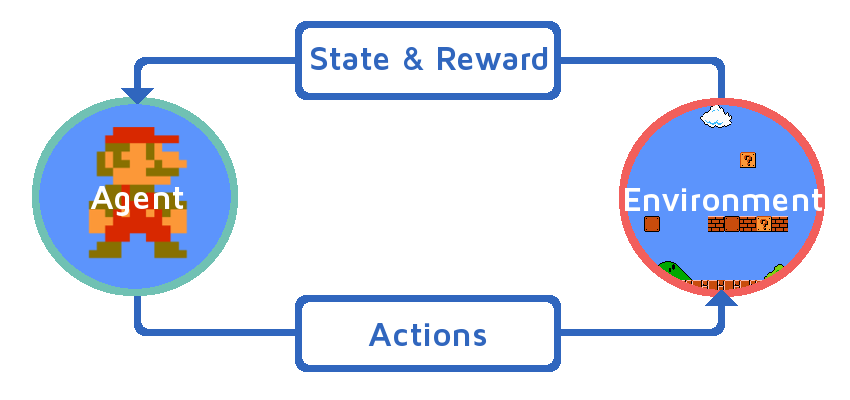
\includegraphics[width=\textwidth]{sty/Mario.png}
\end{frame}

\section{How an agent learns}
\begin{frame}{Types of tasks}
    An instance of a reinforcement learning problem, or a task, may be divided in two types:
    \begin{itemize}
        \item Episodic: when we have an start and an end point. For example playing chess.
        \item Continous: when we have an start but not an explicit end point. For example stock trading
    \end{itemize}
\end{frame}
\begin{frame}{States and Rewards}
    Each state $S_t$ represents the environment at a given time \textit{t} and has associated to it a set of actions $A(S_t)$. $\forall a \in A(S_t)$ we have $r_a \in \mathbb{R}$ representing the reward for that action and also the resulting state $S_{t+1}$. The reward accumulated after a state $S_t$ is called $R_{t+1}$.
\end{frame}
\begin{frame}{Cummulative rewards}
    Reinforcement learn works by maximizing the reward over a number of iterations. 
    For an episodic task, the cumulative reward at a given time \textit{t} can be defined as:
    \[ G_t = \sum_{k=0}^{T} R_{t+k+1} \] 
    For continous tasks, however, this definition does not work, so we define a discount $\gamma \in \left[0,1\right[$, which is a discount applied to each step. The larger the $\gamma$, the smaller the discount:
    \[ G_t = \sum_{k=0}^{\infty} \gamma^k R_{t+k+1} \] 
\end{frame}
\begin{frame}{Value functions}
    Using this idea of cummulative rewards, it is possible to estimate the value of a state as the expected sum of rewards from a given state onward:
    \[ v_\pi (s) =  \mathbb{E} \Big[ \sum_{k=0}^{\infty} \gamma^k R_{t+k+1} \mid S_t=s \Big] \]
\end{frame}
\begin{frame}{Maximizing the reward sum}
    So, given that achieving the goal means to maximize the sum of rewards at a given time we just need to choose the action \textit{a} at a state $S_t$ such that $R_{t+1} \geqslant r_a, \forall a \in A(S_t)$.
\end{frame}
\begin{frame}{Policies}
    By selecting the maximum reward action at each state we end-up by generating a mapping of which action to take at each state. This mapping is called a policy and is usually denoted as $a = \pi(s)$. There may be two types of policies:
    \begin{itemize}
        \item Deterministic: In which for a state \textit{s} there will always have only one maximum action \textit{a}.
        \item Stochastic: Which returns for a state \textit{s} the probability with which the agent should consider action \textit{a}.
    \end{itemize}
\end{frame}

\section{Conclusion}
\begin{frame}{Conclusion}
    So main concept behind reinforcement learning is to look for an optimal policy, which means to learn a sequence of actions an agent must take in order to maximize the sum of rewards over a series of interactions with a given environment
\end{frame}

\nocite{*}

\begin{frame}[allowframebreaks]{References}

  \bibliography{rl}
  \bibliographystyle{abbrv}

\end{frame}

\end{document}
